\documentclass{article}
\usepackage{graphicx}
\usepackage{float}

\begin{document}

\title{CS181 Spring 2016 Practical 2: Classifying Malicious Software | Team EXT3}
\author{Robert J. Johnson | Dinesh Malav | Matthew McKenna}



\maketitle

\begin{abstract}
Identifying and eliminating malicious software (malware) is a modern computing task of considerable importance. Properly classifying these programs in a computationally efficient manner will lead to massive savings in time and money. Our study showed how various machine learning classifiers performed at this task when presented with malicious XML executables. A random forest classifier was shown to be the best model tested, with a categorization accuracy of .81211 on the test data. 
\end{abstract}

\section{Technical Approach}
The training data set for our examination consisted of 3086 XML executable files. Of these, roughly half contained malware. The XML files on first glance appear quite daunting, with large hexadecimal strings and quasi-random calls to various processes intermingled throughout the scripts. Another foundational problem with the data analysis is the nature of the differences between the malware classes. The differences between certain classes are subtle, adding another layer of complexity to the classification process.\\\\
After initial testing of various generative and probabilistic classifiers, it was obvious that proper feature selection would be the primary manner in which we could improve the model. From the XML files, we attempted to extract certain calls in the executable that could be used by malicious software to attack a computer system. These calls were as follows:\\\\
'sleep', 'dump\_line', 'open\_key', 'query\_value', 'load\_dll', 'remove\_directory', 'create\_directory', 'get\_computer\_name', 'open\_url', 'process', 'vm\_protect', 'vm\_allocate', 'create\_mutex'\\\\
Intuitively, these were seen as calls that could manipulate a computer and this were able to be used as accurate classifiers for identifying malware. Utilization of dynamic-link libraries (DLLs) were also seen as a potentially valuable indicator in our classification, and accordingly we added features pertaining to DLL usage. Towards the end of our analysis, we added in code to parse and count the total number of XML tags that occurred in each executable. 
We attempted to use a wide range of classification paradigms in our analysis. The following techniques were used at various points in our study:\\\\
Random Forest Classifier, Quadratic Discriminant Analysis, AdaBoost Classifier,  Gaussian Naive Bayes, Decision Tree Classifier, Support Vector Machine, K-Nearest Neighbor Classifier
\section{Results}
Ultimately, our random forest classifier was the most accurate.  This classifier had an accuracy of .81211 on the test data set on Kaggle. Accuracies of the various models on our own partitioned out test set are below. The full results are charted on the next  page. 
\begin{figure}[h]
\centering
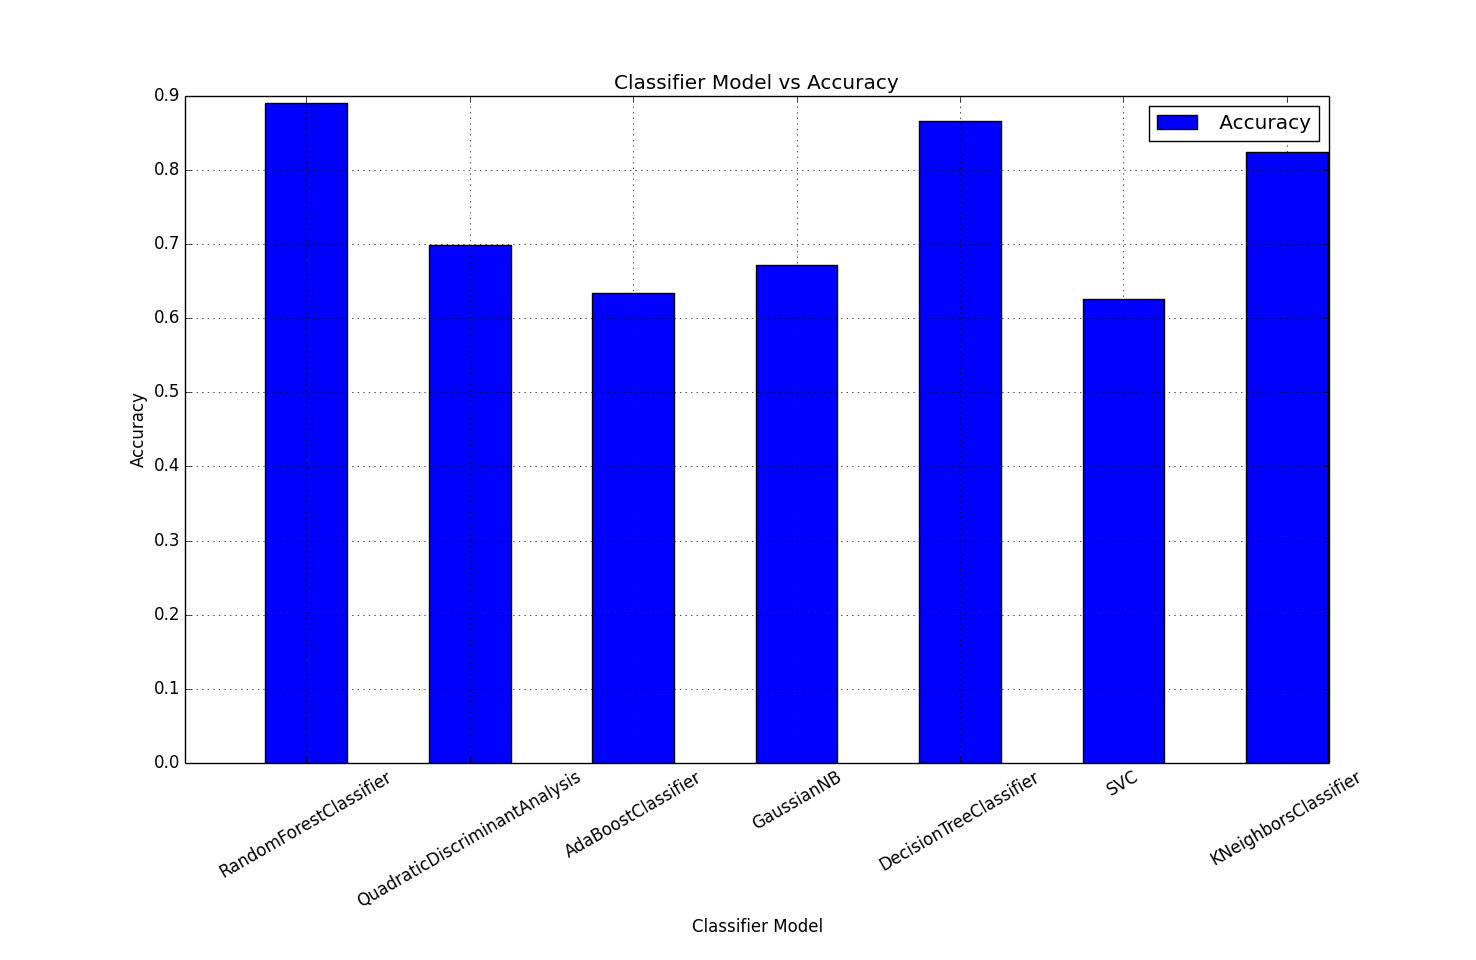
\includegraphics[width=1.0\textwidth]{classifier_selection.png}
\caption{Classifier Model vs Accuracy}
\label{classifier_selection}
\end{figure}\\
\begin{table}[ht]
\centering 
\begin{tabular}{c c } 
\hline 
Method & Accuracy\\ [0.5ex] 
\hline 
Random Forest Classifier & 0.890524379025 \\ 
Quadratic Discriminant Analysis & 0.699172033119\\
AdaBoost Classifier & 0.634774609016\\
Gaussian Naive Bayes & 0.671573137075\\
Decision Tree Classifier & 0.866605335787\\
Support Vector Machine & 0.625574977001\\
K-Nearest Neighbor Classifier & 0.824287028519\\ [1ex] 
\hline 
\end{tabular}
\label{table:nonlin} 
\end{table}\\
The semi-structured nature of the data appears to have led to the success of the Random Forest approach. Random Forest algorithms in general tend to do well with larger datasets with large numbers of features. Once we realized Random Forest Classification was the most accurate model, we attempted to tweak the parameters to improve the accuracy of the model. 
\begin{table}[ht]
\centering 
\begin{tabular}{c c } 
\hline 
Parameters for Random Forest & Accuracy\\ [0.5ex] 
\hline 
n\_estimators=100, max\_features='None' & 0.891444342226\\ 
n\_estimators=50, max\_features='log2' & 0.894204231831\\
n\_estimators=100, max\_features='log2' & 0.897884084637\\
n\_estimators=125, max\_features='log2' & 0.896964121435\\
n\_estimators=115, max\_features='log2' & 0.896044158234\\ [1ex] 
\hline 
\end{tabular}
\label{table:nonlin} 
\end{table}

\section{Discussion}
We found that good feature engineering was again crucial to making accurate predictions, and different classification techniques resulted in significant differences in accuracy. One interesting result was that Random Forest, Decision Tree Classifier, and K-Nearest Neighbor Classifier methods significantly out-performed the other methods tested. The accuracy for these models was in the 82\% - 89\% range, while the other methods were in the 60\%-69\% range.  These three methods are weighted-neighborhood schemes, so it seems this approach was most appropriate for the given data. One reason the Random Forest performed better than other weighted-neighborhood schemes could be because it controls for over-fitting to the training data set, at least compared to the Decision Tree Classifier)\\\\
As we saw in the last practical, different model classes gave fairly different results, but once we found the best model type, fine-tuning the model parameters gave only a slight improvement. Tuning the n\_estimators and max\_features parameters improved the Random Forest accuracy, but only by about 0.1\%. The highest percent accuracy (89.79\%) was achieved with n\_estimators set to 100 and max\_features set to 'log2'.\\\\
Future work could include graphing the percent accuracy as a function of model parameters to find the values that give the highest percent accuracy in the data. Other future work could involve exploring additional Random Forest Classification parameters. Some initial work showed that turning off the 'bootstrap' parameter (i.e. using the entire dataset instead of bootstrapped datasets) slightly improved model accuracy. Also, having a domain expert would be helpful to see which properties of the XML executable files are known to be predictive of malware class. Because most malware class had very low frequencies in the training data (11 of the 15 malware classes had a frequency of less than 2\% in the training data), having a larger dataset would allow us to model these malware classes more accurately, and therefore predict malware class more accurately. Another approach that we were unable to draft due to time constraints was one that analyzed the number of distinct n-grams in the executable files. This method idea is based off of a similar approach taken by J. Ziko Kolter, a professor at Carnegie Mellon, and Marcus Maloof, a professor at Georgetown.\footnote{http://www.jmlr.org/papers/volume7/kolter06a/kolter06a.pdf} Their study compiled over 255 million distinct n-grams and used the data to classify malware with a true positive rate of approximately 98\%. This appears to be an incredibly useful technique in the detection of malware. \\\\
All code for this project can be found at: $$https://github.com/HarvardCS181Practical2016$$.




\end{document}
